\ifthenelse{\equal{\Langue}{FR}}{
    \chapter{Alimentation d'un microprocesseur}
}{
    \chapter{Powering a microprocessor}
}

\ifthenelse{\equal{\Langue}{FR}}{
    On souhaite alimenter un microprocesseur STM32H4 à l'aide d'une batterie. Le cahier des charges est le suivant:
}{
    We want to power an STM32H4 microprocessor using a battery. The specifications are as follows:

}

\begin{itemize}
\ifthenelse{\equal{\Langue}{FR}}{
    \item Batterie LiPo 2S $V_{in} = 7.4\ V$
    \item Tension d'alimentation du microprocesseur: $V_{out}=3.3\ V$
    \item Ondulation de tension max en entrée du microprocesseur: $\Delta V_S = 50\ mV$
    \item Courant nominal de sortie: $I_S = 200\ mA$
    \item Ondulation de courant: 30\%
}{
    \item LiPo 2S battery $V_{in} = 7.4\ V$
    \item Microprocessor supply voltage: $V_{out}=3.3\ V$
    \item Maximum voltage ripple at the microprocessor input: $\Delta V_S = 50\ mV$
    \item Output nominal current: $I_S = 200\ mA$
    \item Current ripple: 30\%
}
\end{itemize}

\ifthenelse{\equal{\Langue}{FR}}{
    Pour cela, on souhaite utiliser le composant suivant: \textbf{LT1959} dont un extrait de la documentation est en annexe. On supposera dans cet exercice que les \underline{\textbf{composants sont}} \underline{\textbf{parfaits}}, et que le Buck fonctionne en régime de \underline{\textbf{conduction continue}}.
}{
    To achieve this, we want to use the following component: \textbf{LT1959}, an excerpt of the documentation is attached. In this exercise, we assume that the \underline{\textbf{components are ideal}}, and that the Buck operates in \underline{\textbf{continuous conduction}} mode.
}

\begin{enumerate}

\ifthenelse{\equal{\Langue}{FR}}{
\item \textbf{Étude du Buck}
}{
\item \textbf{Buck Study}
}

\begin{enumerate}

\ifthenelse{\equal{\Langue}{FR}}{
\item Tracer le circuit permettant d'utiliser ce composant en fonctionnement Buck (la valeur des composants passifs n'est pas demandée). Pour la broche 6 $\overline{SHDN}$, on supposera que le Buck est toujours en fonctionnement.
}{
\item Draw the circuit to use this component in Buck operation (the values of the passive components are not required). For pin 6 $\overline{SHDN}$, assume that the Buck is always operational.
}

\ifthenelse{\equal{\SuCorr}{CO}}{
\begin{center}

\includegraphics[width=0.8\linewidth]{TD_Buck/fig/Q1_1.png}
\end{center}
}


\ifthenelse{\equal{\Langue}{FR}}{
\item On suppose que le processeur absorbe un courant $I_s$ constant égal au courant nominal et que la tension de sortie est constante (on néglige l'ondulation de la tension de sortie). Tracer l'allure de la tension $V_{SW}$ en sortie du composant \textbf{LT1959}, $I_{SW}$ le courant de sortie du composant, la tension $V_{ce}$ aux bornes du transistor $Q_1$ et le courant $I_{L}$ dans l'inductance de sortie. En déduire la relation entre la tension d'entrée $V_{in}$, $V_{out}$ et le rapport cyclique $\alpha$ du hacheur.
}{
\item We assume that the processor draws a constant current $I_s$ equal to the nominal current and that the output voltage is constant (we neglect the output voltage ripple). Plot the waveform of the voltage $V_{SW}$ at the output of the \textbf{LT1959} component, the output current $I_{SW}$, the voltage $V_{ce}$ across the transistor $Q_1$, and the current $I_{L}$ through the output inductor. Deduce the relationship between the input voltage $V_{in}$, $V_{out}$, and the duty cycle $\alpha$ of the converter.
}

\ifthenelse{\equal{\SuCorr}{CO}}{
\begin{center}
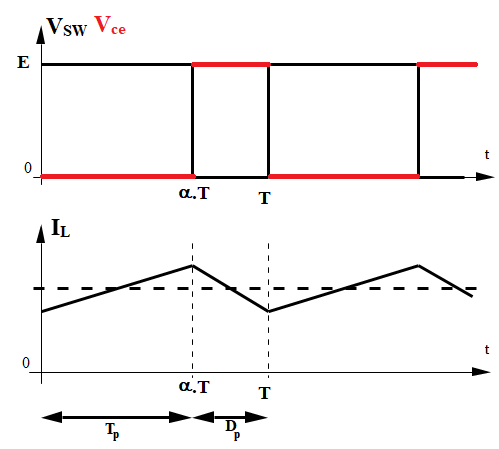
\includegraphics[width=0.7\linewidth]{TD_Buck/fig/Q1_2.png}

$V_{out}=<V_{SW}>=\alpha V_{in}$
\end{center}
}

\ifthenelse{\equal{\Langue}{FR}}{
\item Si la tension de sortie est bien régulée, quelle sera la valeur du rapport cyclique $\alpha_n$ imposé par le \textbf{LT1959}?
}{
\item If the output voltage is well regulated, what will be the value of the duty cycle $\alpha_n$ imposed by the \textbf{LT1959}?
}

\ifthenelse{\equal{\SuCorr}{CO}}{
\begin{center}
$\alpha=\dfrac{V_{out}}{V_{in}}=\dfrac{3.3}{7.4}\approx0.45$
\end{center}
}

\ifthenelse{\equal{\Langue}{FR}}{
\item Justifier que ce composant est adapté au cahier des charges. Peut-on utiliser une batterie LiPo 1S ($3.7 V$) à la place de la LiPo 2S\@?
}{
\item Justify that this component is suitable for the specifications. Can we use a LiPo 1S battery ($3.7 V$) instead of the LiPo 2S\@?
}

\ifthenelse{\equal{\SuCorr}{CO}}{
\begin{center}
\ifthenelse{\equal{\Langue}{FR}}{
Tension d'entrée min: 4 V $\rightarrow V_{in}>4\ V$

Tension de sortie min: 1.21 V $\rightarrow V_{out}>1.21\ V$

Courant de commutation max pour le composant: 4.5 A $\rightarrow$ Courant max à commuter: $I_S+\Delta I_s/2 =0.2+0.2*0.15=0.23<4.5\ A$

LiPo 1S\@: $3.7\ V < 4\ V\ \rightarrow$ ne peut pas fonctionner directement avec ce composant
}{
Minimum input voltage: 4 V $\rightarrow V_{in}>4\ V$

Minimum output voltage: 1.21 V $\rightarrow V_{out}>1.21\ V$

Maximum switching current for component: 4.5 A $\rightarrow$ Maximum current: $I_S+\Delta I_s/2 =0.2+0.2*0.15=0.23<4.5\ A$

LiPo 1S\@: $3.7\ V < 4\ V\ \rightarrow$ cannot operate directly with this component
}
\end{center}
}

\ifthenelse{\equal{\Langue}{FR}}{
\item A partir de la documentation, quelle est la fréquence de découpage du hacheur?
}{
\item Based on the documentation, what is the switching frequency of the converter?
}

\ifthenelse{\equal{\SuCorr}{CO}}{
\begin{center}
$f_{SW}=500\ kHz$
\end{center}
}

\ifthenelse{\equal{\Langue}{FR}}{
\item Calculer l'ondulation de courant $\Delta I_{L}$ dans l'inductance de sortie, en fonction de l'inductance $L_1$ placée. En déduire la valeur de l'inductance afin de respecter le cahier des charges.
}{
\item Calculate the current ripple $\Delta I_{L}$ through the output inductor, as a function of the inductance $L_1$ used. Deduce the value of the inductance to meet the specifications.
}

\ifthenelse{\equal{\SuCorr}{CO}}{
\begin{center}
\ifthenelse{\equal{\Langue}{FR}}{
Entre 0 et $\alpha T$: $V_L=V_{in}-V_{out}=L\dfrac{dI_L}{dt} \rightarrow \Delta I_L=(V_{in}-V{out}).\dfrac{\alpha T}{L}$
}{
Between 0 and $\alpha T$: $V_L=V_{in}-V_{out}=L\dfrac{dI_L}{dt} \rightarrow \Delta I_L=(V_{in}-V{out}).\dfrac{\alpha T}{L}$
}
$\Delta I_L=\dfrac{\alpha .(1-\alpha).V_{in}.T}{L}$

$L>61\mu H$
\end{center}
}

\ifthenelse{\equal{\Langue}{FR}}{
\item Tracer la tension de sortie en tenant compte de l'ondulation de tension. Calculer la valeur du condensateur de sortie $C_1$ à choisir afin de respecter le cahier des charges.
}{
\item Plot the output voltage taking into account the voltage ripple. Calculate the value of the output capacitor $C_1$ to choose in order to meet the specifications.
}

\ifthenelse{\equal{\SuCorr}{CO}}{
\begin{center}
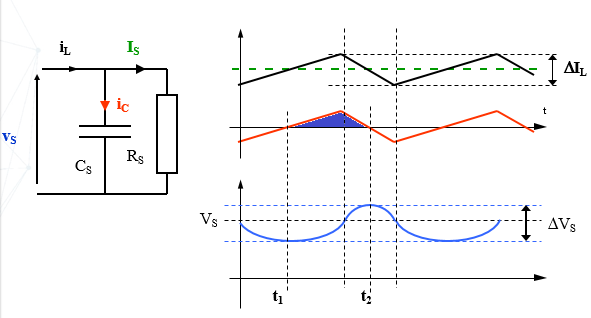
\includegraphics[width=0.7\linewidth]{TD_Buck/fig/Q1_7.png}

\[t_1=\dfrac{\alpha.T}{2}\ \ \ \ \  t_2=\dfrac{(1+\alpha).T}{2}\]

\[\Delta V_C=\dfrac{1}{C_1}\int_{t_1}^{t_2}i_C(t).dt=\dfrac{1}{C_1}.\dfrac{1}{2}.\dfrac{\Delta I_S}{2}.(t_2-t_1)\]

\[\rightarrow C_S=\dfrac{\alpha.(1-\alpha).V_{in}}{8.f_{SW}^2.L.\Delta V_S}=300\ nF\]
\end{center}
}

\ifthenelse{\equal{\Langue}{FR}}{
\item Que se passe-t-il si le microprocesseur consomme peu de courant (mode veille par exemple)?
}{
\item What happens if the microprocessor consumes very little current (e.g., sleep mode)?
}

\ifthenelse{\equal{\SuCorr}{CO}}{
\begin{center}
\ifthenelse{\equal{\Langue}{FR}}{
Conduction discontinue $\rightarrow$ si $\alpha$ est fixe, $V_S$ augmente (potentiellement jusqu'à $V_{in}=7.4\ V$ si le processeur ne consomme aucun courant)
}{
Discontinuous conduction mode $\rightarrow$ if $\alpha$ is fixed, $V_S$ increases (potentially up to $V_{in}=7.4\ V$ if the processor consumes no current)
}
\end{center}
}

\end{enumerate}



\ifthenelse{\equal{\Langue}{FR}}{
\item \textbf{Etude de la commande}

Dans cette partie, on s'intéresse à la commande du Buck. Pour cela, on utilise le schéma simplifié suivant:
}{
\item \textbf{Control Study}

In this part, we are interested in the control of the Buck converter. For this purpose, we use the following simplified schematic:
}

\begin{figure}[ht]
\centering
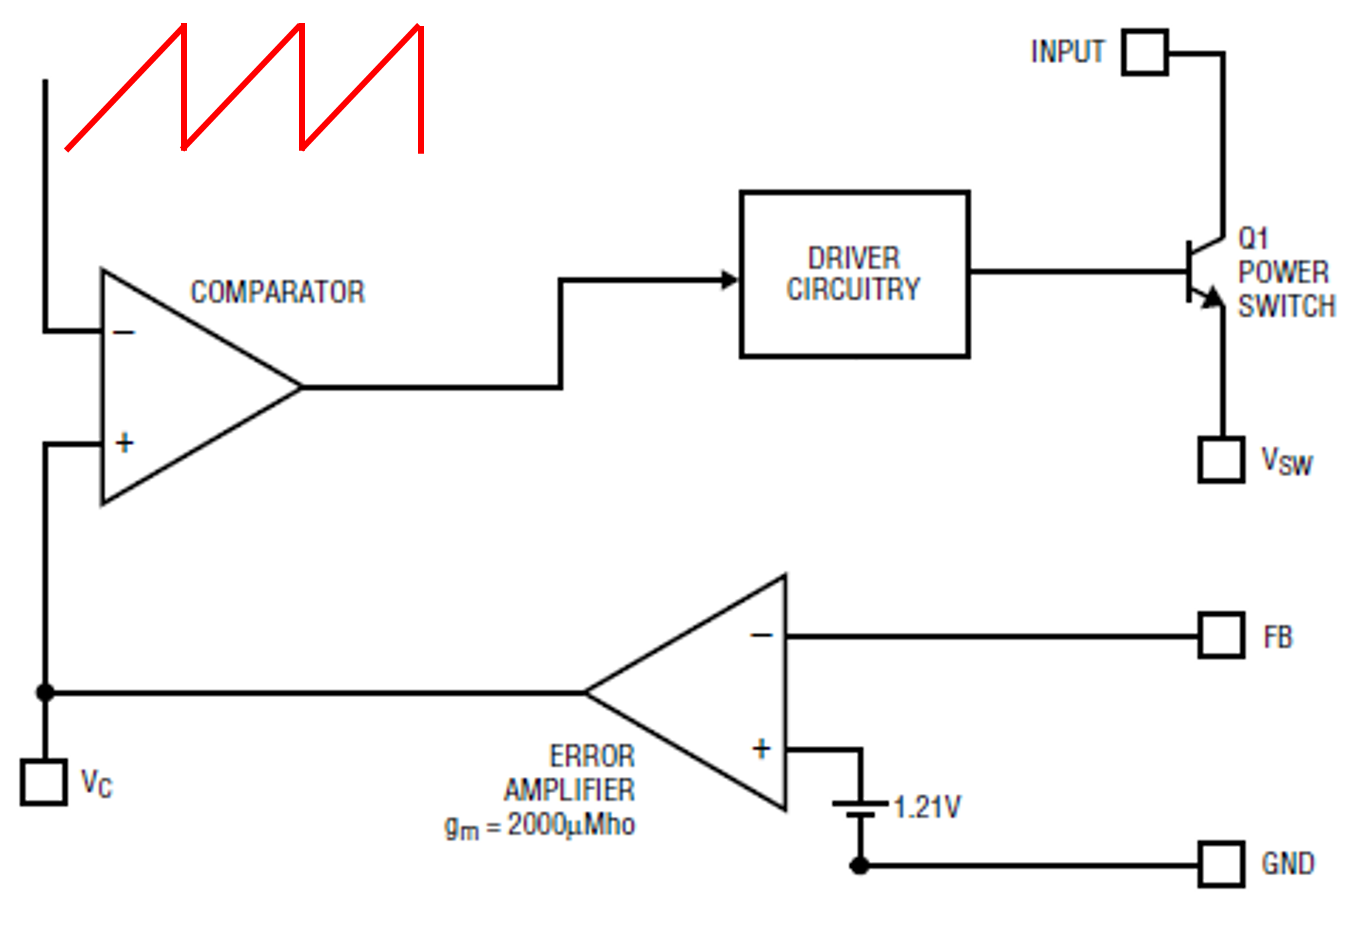
\includegraphics[width=0.8\linewidth]{TD_Buck/fig/Buck_regul.png}
\caption{Simplified internal control}
\end{figure}


\ifthenelse{\equal{\Langue}{FR}}{
Le signal en dent de scie évolue entre 0 et 2 V, avec une fréquence égale à la fréquence de découpage du hacheur. 
}{
The sawtooth signal varies between 0 and 2 V, with a frequency equal to the switching frequency of the converter.
}

\begin{enumerate}

\ifthenelse{\equal{\Langue}{FR}}{
\item Calculer la valeur de la résistance $R_1$ à connecter sur la broche \textit{FB} afin d'avoir la tension de sortie demandée, sachant qu'on choisit $R_2=2.7k\Omega$. Vérifier que la valeur de $R_1$ est bien dans la série E12.

(Valeurs de la série E12: 100, 120, 150, 180, 220, 270, 330, 390, 470, 560, 680, 820).
}{
\item Calculate the value of the resistor $R_1$ to connect to the \textit{FB} pin in order to have the desired output voltage, knowing that we choose $R_2=2.7k\Omega$. Verify that the value of $R_1$ is indeed in the E12 series.

(E12 series values: 100, 120, 150, 180, 220, 270, 330, 390, 470, 560, 680, 820).
}

\ifthenelse{\equal{\SuCorr}{CO}}{
\begin{center}
\ifthenelse{\equal{\Langue}{FR}}{
Pont diviseur de tension: $\dfrac{R_2}{R_1+R_2}=\dfrac{1.21}{3.3}\rightarrow R_1\approx 1.73.R_2$
}{
Voltage divider: $\dfrac{R_2}{R_1+R_2}=\dfrac{1.21}{3.3}\rightarrow R_1\approx 1.73.R_2$
}
\[R_1=4.7\ k\Omega\]
\end{center}
}

\ifthenelse{\equal{\Langue}{FR}}{
\item Pour une tension $V^+=0.5 V$ à l'entrée du comparateur, tracer le signal en sortie du comparateur. En déduire l'expression qui lie la tension $V^+$ du comparateur et la valeur du rapport cyclique $\alpha$ du hacheur.
}{
\item For an input voltage $V^+=0.5 V$ at the comparator input, plot the output signal of the comparator. Deduce the expression that relates the comparator voltage $V^+$ and the duty cycle $\alpha$ of the converter.
}

\ifthenelse{\equal{\SuCorr}{CO}}{
\begin{center}
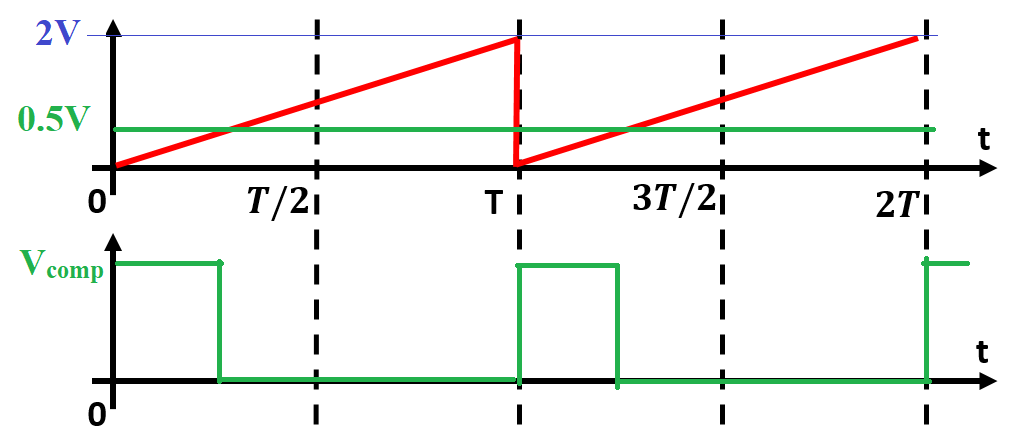
\includegraphics[width=0.7\linewidth]{TD_Buck/fig/Q2_1.png}
\[V^+=2.\alpha\]
\end{center}
}

\ifthenelse{\equal{\Langue}{FR}}{
On modélise le convertisseur asservi avec le schéma bloc suivant:
}{
The controlled converter is modeled with the following block diagram:
}

\begin{figure}[H]
\centering
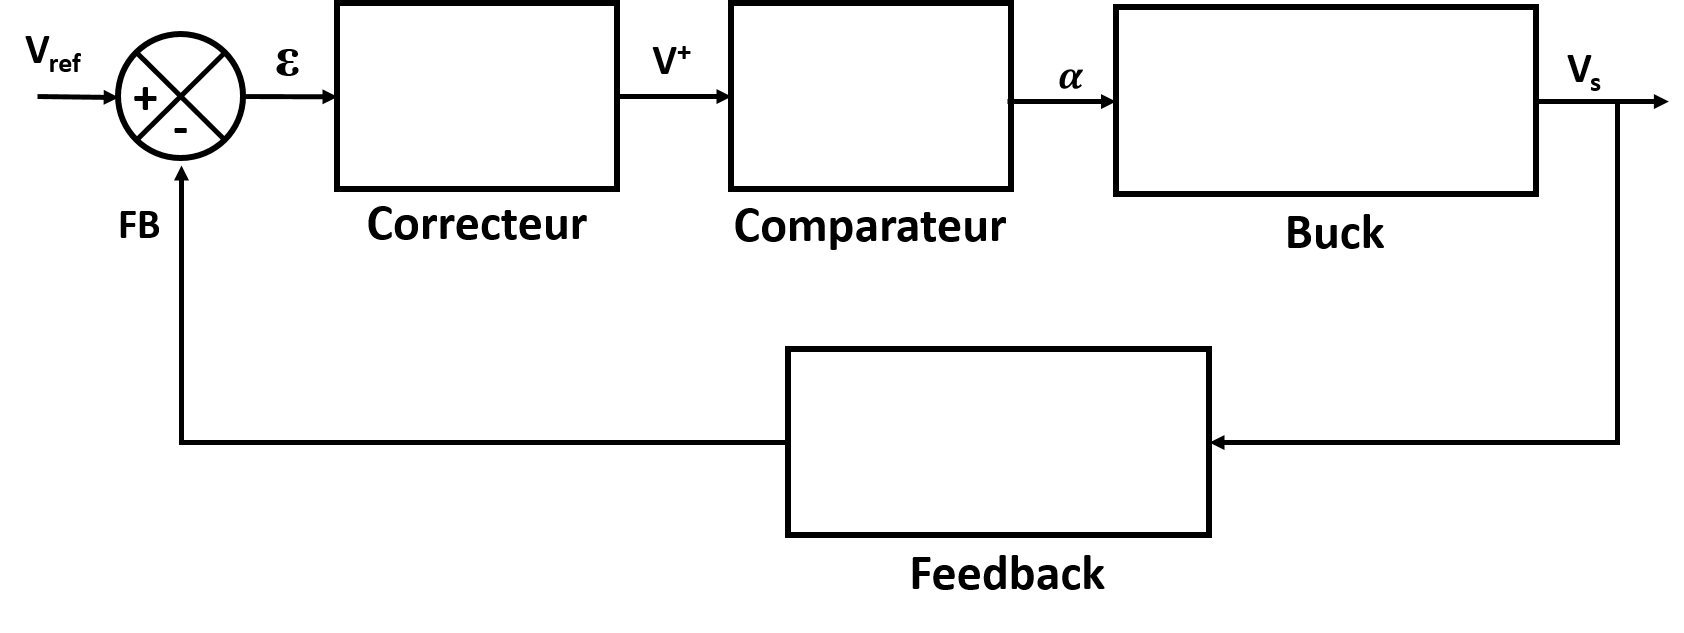
\includegraphics[width=0.8\linewidth]{TD_Buck/fig/Buck_regul_1.png}
\caption{Global bloc diagramm}
\end{figure}


\ifthenelse{\equal{\Langue}{FR}}{
\item Compléter le bloc ``\textit{Comparateur}''. A l'aide de la partie 1, compléter le bloc ``\textit{Feedback}''

Le bloc ``\textit{Buck}'' est modélisé par un gain statique $K$ correspondant à $\dfrac{V_{s\ moy}}{\alpha}$ et une fonction de transfert correspondant au filtre de sortie de Buck. La résistance $R_m$ symbolise l'impédance d'entrée du microcontrôleur.
}{
\item Complete the ``\textit{Comparator}'' block. Using part 1, complete the ``\textit{Feedback}'' block.

The ``\textit{Buck}'' block is modeled by a static gain $K$ corresponding to $\dfrac{V_{s\ avg}}{\alpha}$ and a transfer function corresponding to the Buck output filter. The resistance $R_m$ represents the input impedance of the microcontroller.
}

\begin{figure}[ht]
\centering
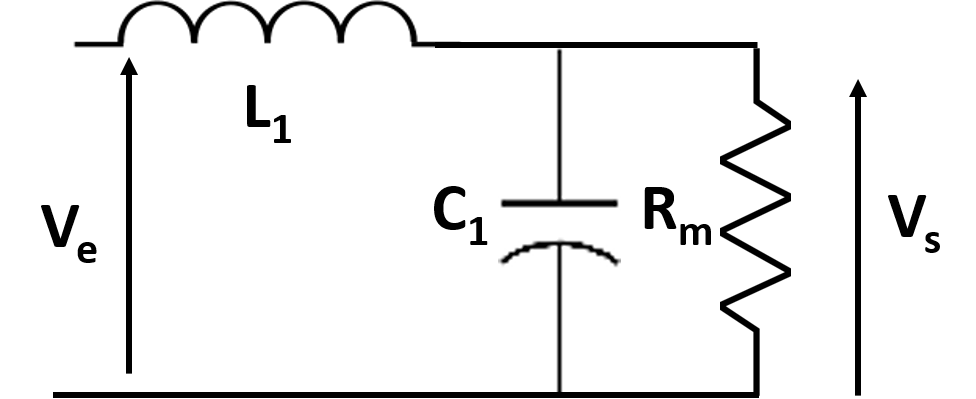
\includegraphics[width=0.55\linewidth]{TD_Buck/fig/Buck_filtre.png}
\caption{Equivalent schematic of the Buck}
\end{figure}

\ifthenelse{\equal{\Langue}{FR}}{
\item Rappeler les valeurs de $L$ et $C$ déterminées à la partie. Déterminer la valeur de $R_m$ lorsque le microcontrôleur absorbe le courant nominal.
}{
\item Recall the values of $L$ and $C$ determined in part 1. Determine the value of $R_m$ when the microcontroller draws the nominal current.
}

\ifthenelse{\equal{\SuCorr}{CO}}{
\begin{center}

$L=61\ \mu H\ \ \ \ \ \ C=300\ nF$

$R_m=\dfrac{V_{out}}{I_S}=16.5\ \Omega$
\end{center}
}

\ifthenelse{\equal{\Langue}{FR}}{
\item Déterminer la fonction de transfert correspondant au bloc ``\textit{Buck}''.
}{
\item Determine the transfer function corresponding to the ``\textit{Buck}'' block.
}

\ifthenelse{\equal{\SuCorr}{CO}}{
\begin{center}
$\dfrac{V_s}{V_e}=\dfrac{1}{1+j.\frac{L_1}{R_m}.\omega-L_1.C_1.\omega^2}$

Buck transfert function: $\dfrac{V_s}{\alpha}=\dfrac{V_{in}}{1+j.\frac{L_1}{R_m}.\omega-L_1.C_1.\omega^2}$
\end{center}
}

\ifthenelse{\equal{\Langue}{FR}}{
\item On place sur la broche $V_c$ un circuit $RC$ série. On suppose que le courant en entrée du comparateur est nul (haute impédance d'entrée). Le bloc ``\textit{Correcteur}'' est donc un proportionnel intégral de la forme $C(p) = K_p(1+\dfrac{1}{T_i.p})$. Déterminer les valeurs de $K_p$ et $T_i$ en fonction de $R$, $C$ et $g_m$.
}{
\item A series $RC$ circuit is placed on the $V_c$ pin. We assume that the input current of the comparator is zero (high input impedance). Therefore, the ``\textit{Corrector}'' block is a proportional integral controller of the form $C(p) = K_p(1+\dfrac{1}{T_i.p})$. Determine the values of $K_p$ and $T_i$ in terms of $R$, $C$, and $g_m$.
}

\ifthenelse{\equal{\SuCorr}{CO}}{
\begin{center}
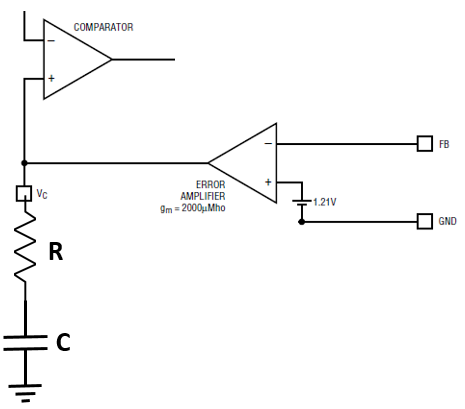
\includegraphics[width=0.55\linewidth]{TD_Buck/fig/Q2_6.png}
$V^+(j\omega)=(R+\dfrac{1}{j.C.\omega}).I(j\omega)=(R+\dfrac{1}{j.C.\omega}).g_m.\epsilon(j\omega)$

$\dfrac{V^+}{\epsilon}=(R+\dfrac{1}{j.C.\omega}).g_m=R.g_m.(1+\frac{1}{j.R.C.\omega})$

$K_p=R.g_m\ \ \ \ \ \ \ \ \ \ \ \ T_i=R.C$
\end{center}
}

\ifthenelse{\equal{\Langue}{FR}}{
\item Calculer $R$ afin que le rapport cyclique au démarrage soit environ égal à $\dfrac{\alpha_n}{2}$ et $C$ pour avoir une constante de temps du correcteur 10 fois supérieure à la constante de temps du système non corrigé.
}{
\item Calculate $R$ so that the duty cycle at startup is approximately equal to $\dfrac{\alpha_n}{2}$ and $C$ to have a time constant of the controller 10 times greater than the time constant of the uncontrolled system.
}

\ifthenelse{\equal{\SuCorr}{CO}}{
\begin{center}
\ifthenelse{\equal{\Langue}{FR}}{
Au démarrage: $V_{FB}=0$ et le condensateur est déchargé: $V^+=R.g_m.\epsilon=1.2R.g_m$

$\alpha=0.5*1.2R.g_m\rightarrow R=\dfrac{\alpha}{0.6g_m}=186\Omega$

Constante de temps du correcteur: $T_i=R.C>10\sqrt{L_1.C_1}\rightarrow C>\dfrac{10}{R}.\sqrt{L_1.C_1}=230\ nF$
}{
At startup: $V_{FB}=0$ and the capacitor is discharged: $V^+=R.g_m.\epsilon=1.2R.g_m$

$\alpha=0.5*1.2R.g_m\rightarrow R=\dfrac{\alpha}{0.6g_m}=186\Omega$

Time constant of the controller: $T_i=R.C>10\sqrt{L_1.C_1}\rightarrow C>\dfrac{10}{R}.\sqrt{L_1.C_1}=230\ nF$
}
\end{center}
}

\ifthenelse{\equal{\Langue}{FR}}{
\item En régime établi, déterminer le courant de sortie de l'ampli d'erreur et les tensions aux bornes de $R$, $C$ et $V_c$. En déduire le rapport cyclique et comparer au résultat du 1.3.
}{
\item In steady state, determine the output current of the error amplifier and the voltages across $R$, $C$, and $V_c$. Deduce the duty cycle and compare it to the result of 1.3.
}

\ifthenelse{\equal{\SuCorr}{CO}}{
\ifthenelse{\equal{\Langue}{FR}}{
Quand t$->$ $\infty$, $\epsilon -> 0$ (thérome de la valeure finale) donc le courant de sortie de l'ampli est nul. 

On a donc $V_{FB}=1.21\ V$ soit $V_{out}=3.3\ V$ comme désiré.

De même, théorme de la valeure finale, $\alpha$ tend vers $\dfrac{R_1+R_2}{R_2}.\dfrac{V_{ref}}{V_{in}}=0.44$
}{
When t$->$ $\infty$, $\epsilon -> 0$ (theorem of the final value) therefore the output current of the amplifier is zero.

We have therefore $V_{FB}=1.21\ V$ so $V_{out}=3.3\ V$ as desired.

Similarly, the theorem of the final value shows that $\alpha$ tends towards $\dfrac{R_1+R_2}{R_2}.\dfrac{V_{ref}}{V_{in}}=0.44$
}
}

\end{enumerate}

\end{enumerate}

\newpage
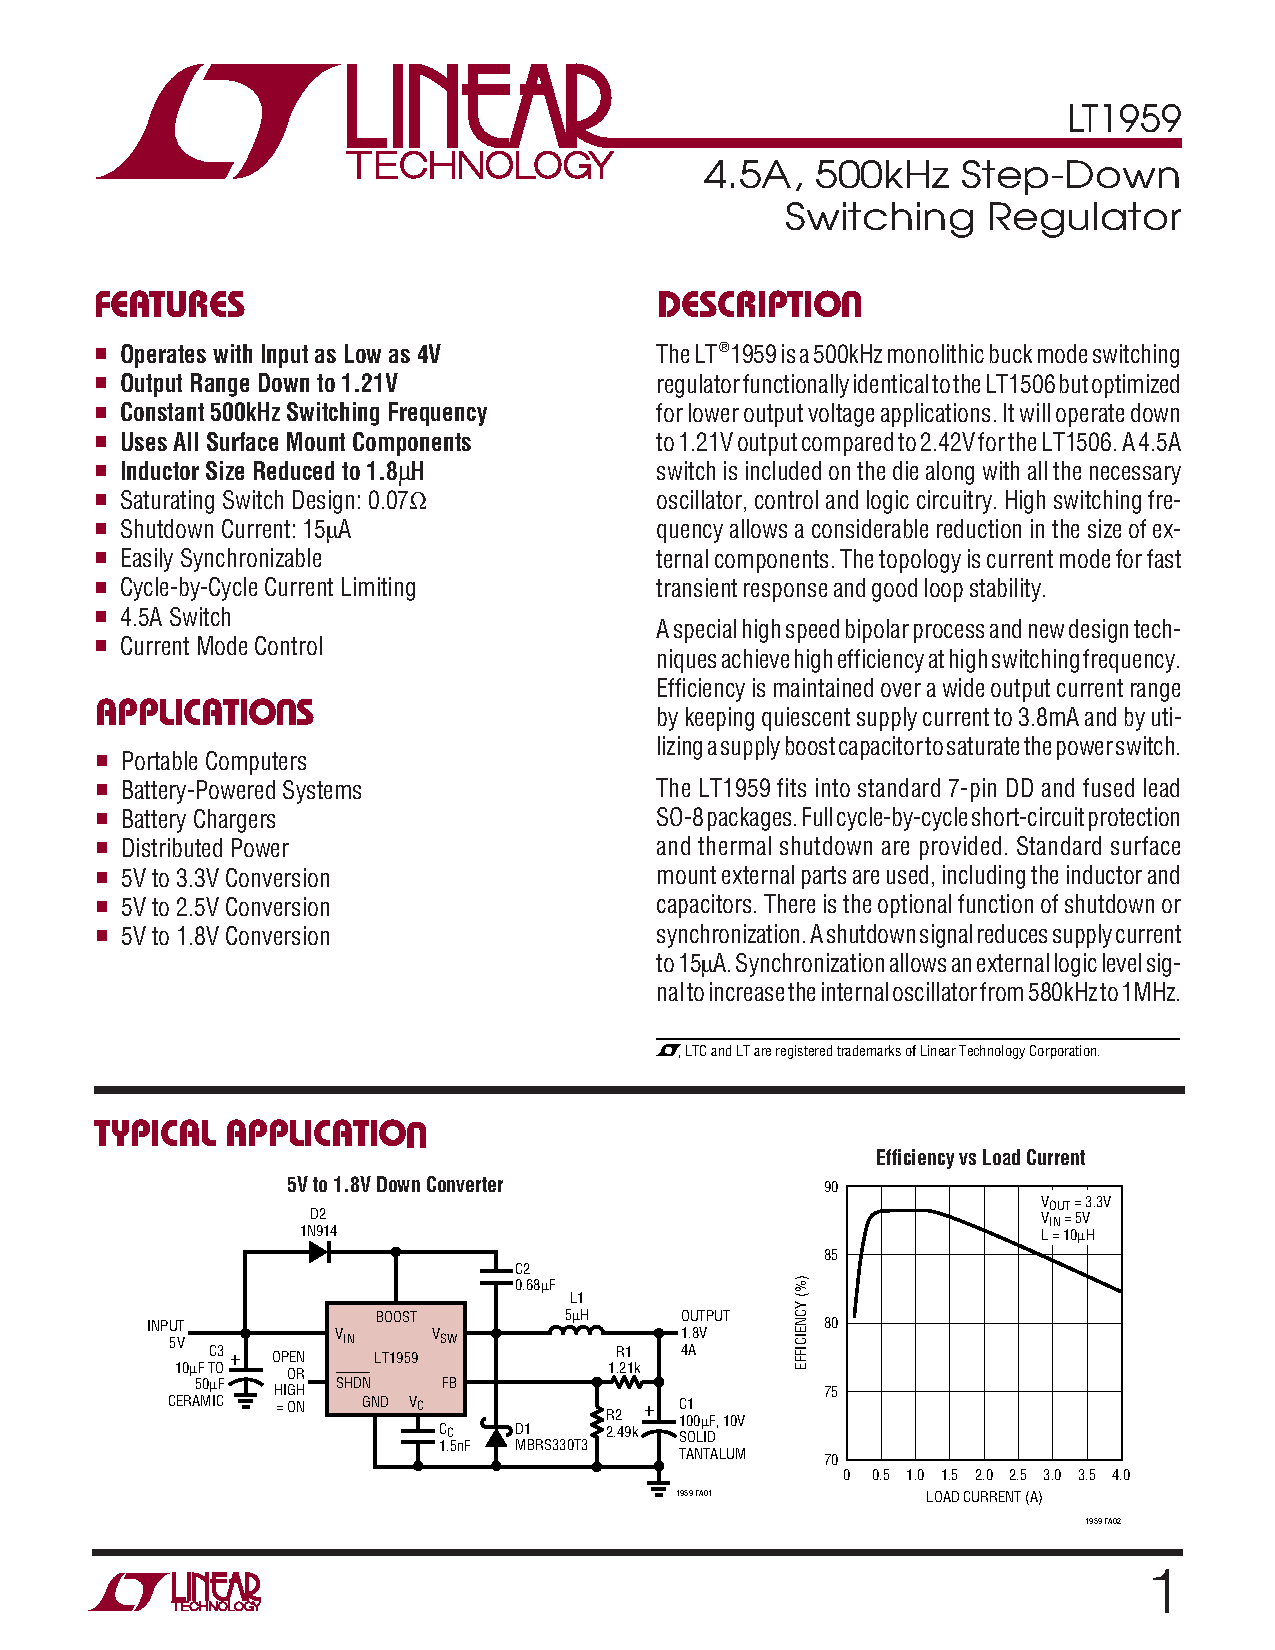
\includepdf[pages={1,2,3,4}]{TD_Buck/fig/LT1959.pdf}
\includepdf[pages={6,7}]{TD_Buck/fig/LT1959.pdf}